\section{Hand detection}\label{sec:hand-detection}
With the advent of the era of augmented reality and virtual reality, the demand for virtual or semi-virtual interfaces
that do not require physical hardware to be used is growing more and more, and one of the most common methods of using
these interfaces is through the use of the hands, the most natural way we have of interacting with our surroundings.

In order to develop these types of interfaces so that they are reliable and comfortable to use,
there is a need for precise methods for detecting hands in a two- or three-dimensional space,
which can understand their positioning and interpret their gestures.

\subsection{MediaPipe}\label{subsec:mediapipe}
MediaPipe is an open-source framework developed by Google for multimodal processing of data streams.
Its flexibility and power make it an ideal tool for developing virtual reality and augmented reality applications.
MediaPipe allows the creation of modular pipelines that can be used in various applications such as facial recognition,
object tracking, hand detection and many others.

\subsubsection{Origin and history}
MediaPipe started as an internal solution to manage and standardise the various computer vision algorithms used in their products.
In 2019~\cite{mediapipe}, Google decided to make MediaPipe an open-source project,
allowing the developer community to contribute and exploit the potential of the platform.
Since its release, MediaPipe has seen rapid adoption due to its ability to simplify development.

\subsubsection{Components and architecture}
MediaPipe's architecture is based on a modular design that allows developers to combine various components to create customised pipelines.
The main components of MediaPipe include:
\begin{itemize}
	\item \textit{Calculator:} it is the fundamental unit of calculation that perform specific operations on data.
	Each calculator receives an input, processes the data and produces an output.
	\item \textit{Graph:} it is a network of calculators that defines the flow of data.
	The graph determines how the data is transformed and transferred between the various calculators.
	\item \textit{Packet:} it is the data transport unit in the graph.
	Packets may contain any type of data, such as images, videos or processing results.
	A particular type of packet is the side packet, a packet without a timestamp that can be used to transport data
	that remain constant, unlike a stream that represents a flow of data that changes over time.
\end{itemize}

\paragraph{Pipeline}
A MediaPipe pipeline is essentially a graph of calculators.
This modular design allows the construction of highly customisable pipelines.
For example, a hand detection pipeline may include calculators for image pre-processing,
hand detection, tracking of key points and post-processing of results.
MediaPipe provides a number of predefined calculators,
but developers can also create their own calculators~\cite{calculators-can-be-created} for specific application needs.
The main components of MediaPipe are:
\begin{itemize}
	\item \textit{Input Streams:} these are sources of data such as video feeds, audio inputs, or sensor data.
	\item \textit{Processing Nodes:} these nodes perform specific tasks like image transformation, feature extraction,
	and machine learning model inference.
	\item \textit{Output Streams:} the processed data is outputted for use in applications,
	such as displaying detected hand gestures or controlling a robotic arm.
\end{itemize}

\paragraph{Hand recognition}
One of the most advanced and popular features of MediaPipe is hand recognition~\cite{mediapipe-hands}.
This feature is designed to be accurate and fast,
working in real time even on mobile devices~\cite{mediapipe-lens-characteristics, mediapipe-sign-language}.
MediaPipe's hand recognition pipeline consists of several steps:
\begin{itemize}
	\item \textit{Hand Detection:} it uses a machine learning model to identify the presence of hands in an image.
	This model is optimised to identify hands in various positions and orientations.
	\item \textit{Landmarks Localization:} once the hand is detected,
	another machine learning model tracks 21 specific landmarks of the hand,
	which include the positions of the finger and palm joints in 2.5D\@.
	The landmarks used by MediaPipe are shown in \autoref{fig:mediapipe-hand-landmarks}
	\item \textit{Post-Processing:} landmark data can be further processed for specific applications,
	such as gesture recognition or interaction with virtual user interfaces.
\end{itemize}
MediaPipe's hand detection model has been trained on a large dataset to ensure high accuracy and robustness.
The pipeline is optimised to run in real time, making it suitable for interactive applications such as
augmented reality games and gesture-based controls.

\begin{figure}[ht]
	\centering
	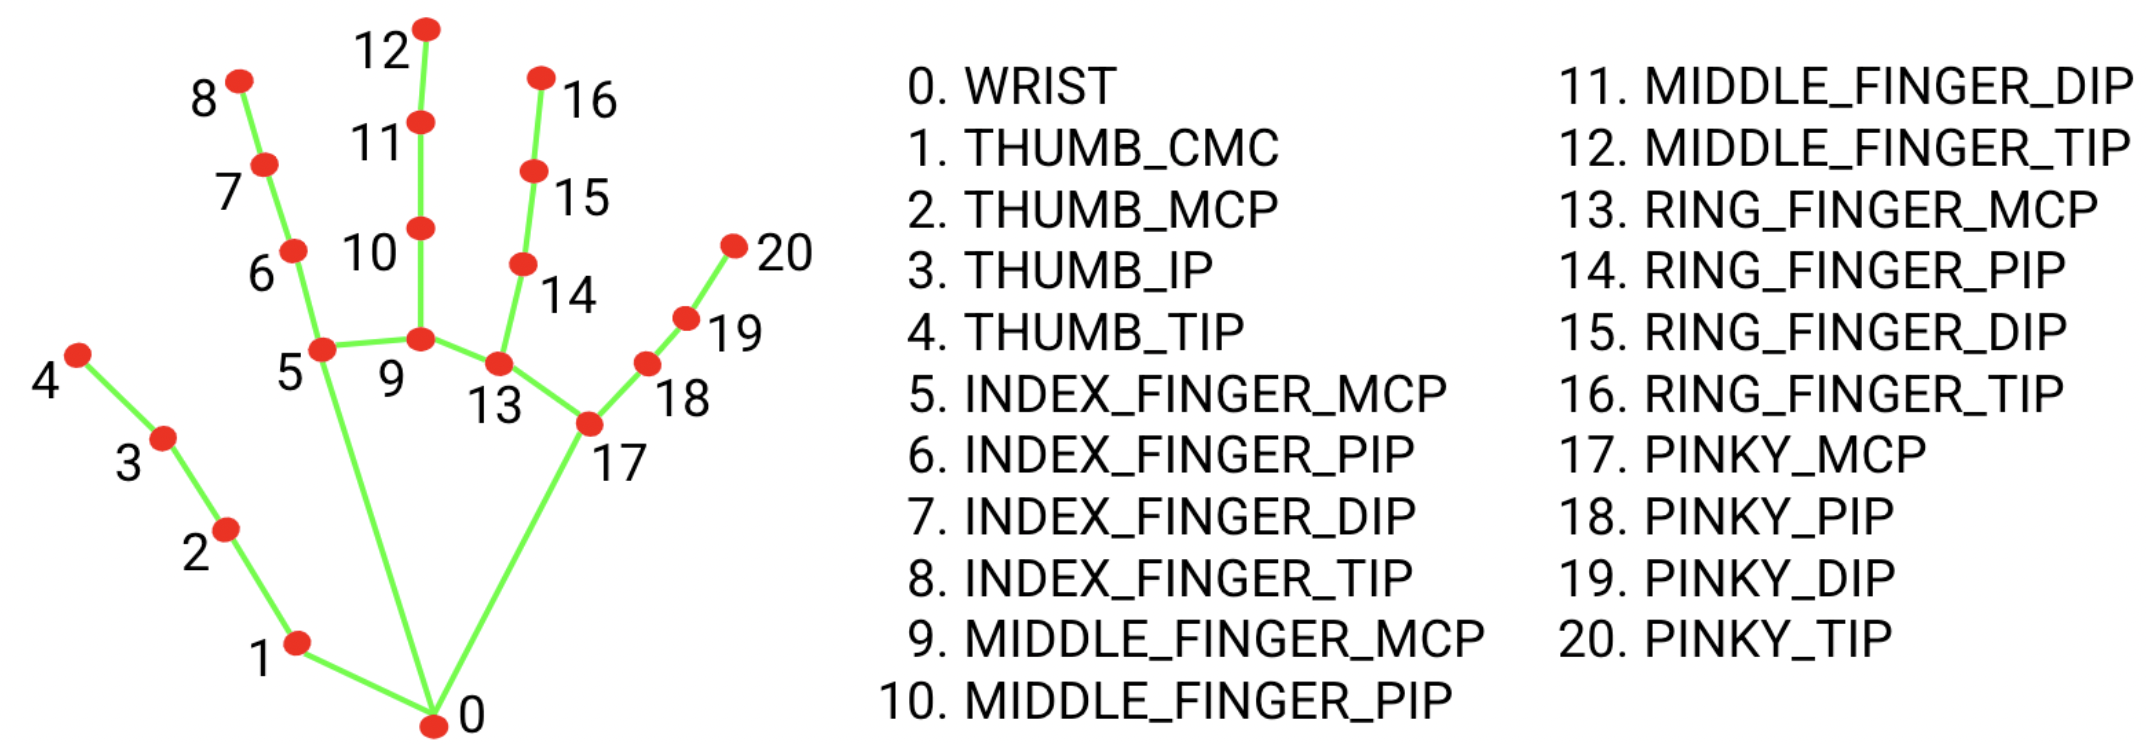
\includegraphics[width=\textwidth]{mediapipe-hand-landmarks}
	\caption{MediaPipe Hand Landmarks}
	\label{fig:mediapipe-hand-landmarks}
\end{figure}

\subsection{ManoMotion}\label{subsec:manomotion}
ManoMotion is an advanced hand gesture recognition technology that fits into the field of augmented reality and virtual reality.
Founded in 2015, ManoMotion's main goal is to provide intuitive and natural interaction between humans
and digital devices through real-time detection of hand movements.

\paragraph{Features}
ManoMotion offers several advanced features that make its hand gesture detection technology particularly useful:

\begin{itemize}
	\item \textit{3D movement recognition:} the technology is able to track hand movements in three dimensions,
	detecting not only the position, but also the depth and orientation of the hands.
	\item \textit{Complex gesture recognition:} ManoMotion can recognise a wide range of complex gestures,
	including finger movements, grasps and releases, rotations and more.
	\item \textit{AR and VR integration:} ManoMotion is designed to easily integrate with leading AR and VR development
	platforms, such as Unity and AR Foundation, facilitating adoption by developers.
	\item \textit{Real-time analysis:} ManoMotion's algorithms process data in real time,
	ensuring a smooth interaction with no perceptible delays.
	\item \textit{Compatibility with mobile devices:} one of the main innovations of ManoMotion is the ability
	to operate on mobile devices, using standard cameras built into phones and tablets.
\end{itemize}

\paragraph{Smartphone}
The way ManoMotion works on a smartphone is particularly impressive: it relies on a remote computing system
in which the smartphone continuously sends the camera's video stream to the ManoMotion server,
which then performs hand and gesture recognition and sends them back to the smartphone in real time.

This method involves shifting the computational load from the smartphone to the ManoMotion servers,
leaving the smartphone with the sole task of transmitting the video stream to the server.
ManoMotion certainly requires a stable and fairly fast connection
(note that the frames sent by the smartphone are not in high resolution anyway),
but it results in a huge reduction in computational load on the part of the smartphone.

This makes ManoMotion particularly suitable for the development of educational applications,
thus intended to be in a classroom, where a school Wi-Fi could be available for use.
An example is the work done in~\cite{manomotion-agilest},
in which ManoMotion is used to create an educational application for chemistry.
This application uses real-time touchless interaction for
kinesthetic and machine learning with a dual purpose: teacher and student evaluator.

\begin{figure}[ht]
	\centering
	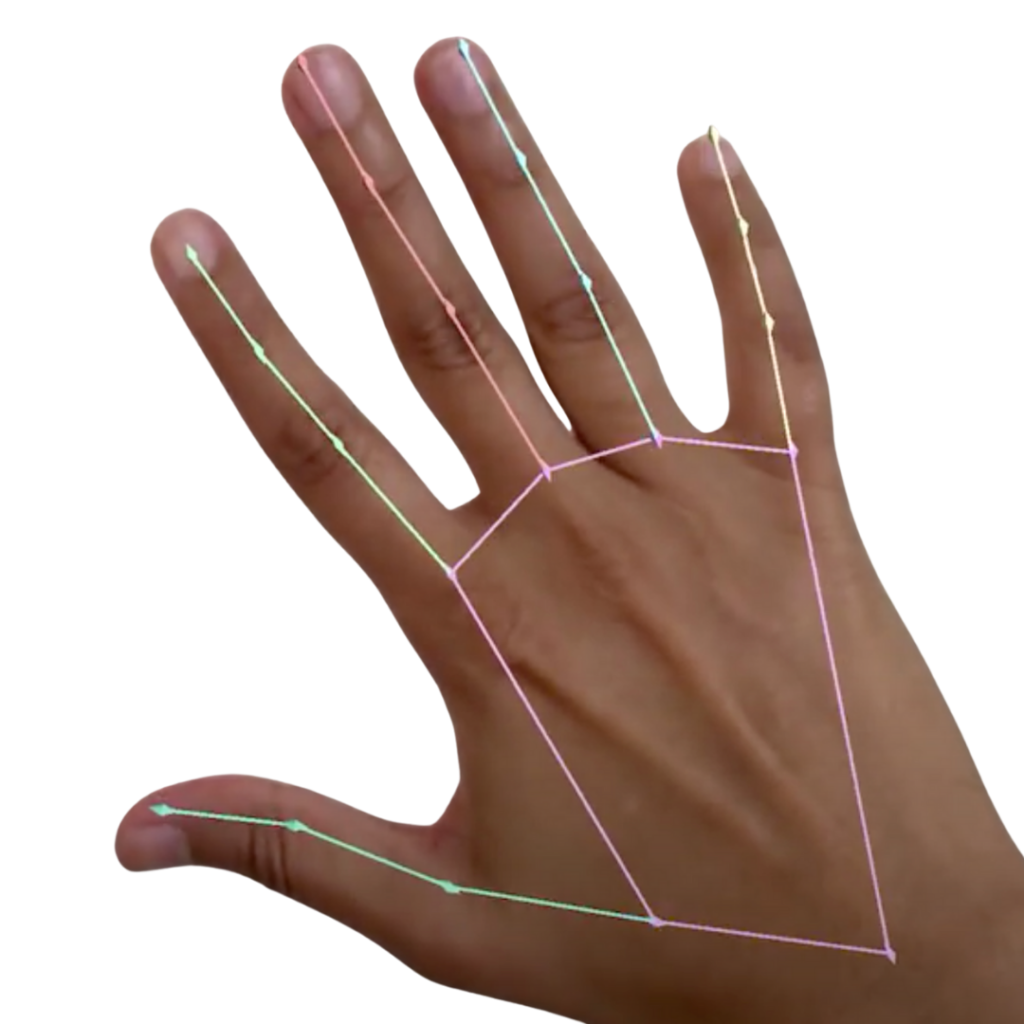
\includegraphics[width=0.5\textwidth]{manomotion-hand}
	\caption{ManoMotion hand skeleton}
	\label{fig:manomotion}
\end{figure}
